% ==================================================%
% Basic setup starts here
%==================================================%
\documentclass[12pt, letterpaper]{amsart} % this will automatically load amsmath and amsthm packages
\usepackage{amsfonts}
\usepackage{amscd} % a CD environment for commutative rectangular diagram
\usepackage{mathtools} % for \shortintertext
\usepackage[utf8]{inputenc} % encoding method
\usepackage[mathscr]{eucal} % eucal calligraphy, mathsrc = use \mathcal
\usepackage{indentfirst} % indent first line of all sections
\usepackage{graphicx} % extension of graphics, options for \includegrahpicx
\usepackage{pict2e} % new implementation of the picture environment, which allows programming pictures directly LaTeX
\usepackage{epic} % add some command to the picture environment
\usepackage[margin=2.9cm]{geometry} % customize page layout
%==================================================%
% Additional setup ends here
%==================================================%
% Additional package used for relevant article
\usepackage{physics} % partial derivative \pdv
\usepackage{cleveref} % automatically add eq in referencing
\usepackage{cancel}
\usepackage{tikz}
\usepackage{float}
% SELF-DEFINED THEOREM using amsthm package
\newtheorem{Th}{Theorem}[section]
\numberwithin{equation}{section}
\newtheorem{Def}[Th]{Definition}
%==================================================%
% Document starts here
% ==================================================%
\author{Kin Chang \\ 304-845-848}
\title{EE183 // Lab 1}
\begin{document}
\maketitle
\section{Introduction}
\begin{center}
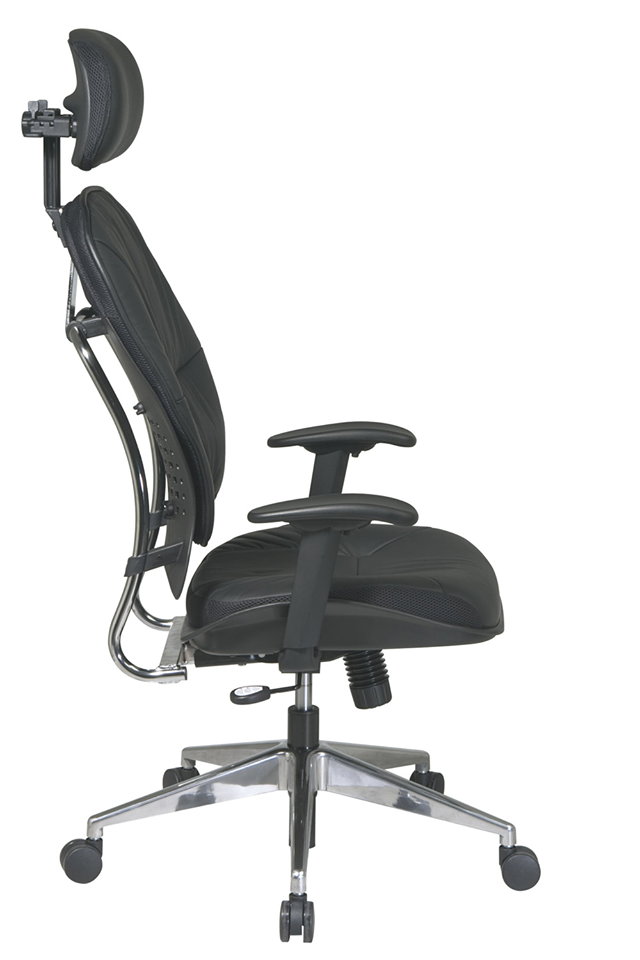
\includegraphics[scale=0.5]{1}  
\end{center}
In this lab, we model a chair with 4 joints with end effector being the headrest. A simplified model schematic of the robot is shown below,
\begin{figure}[H]
  \centering
  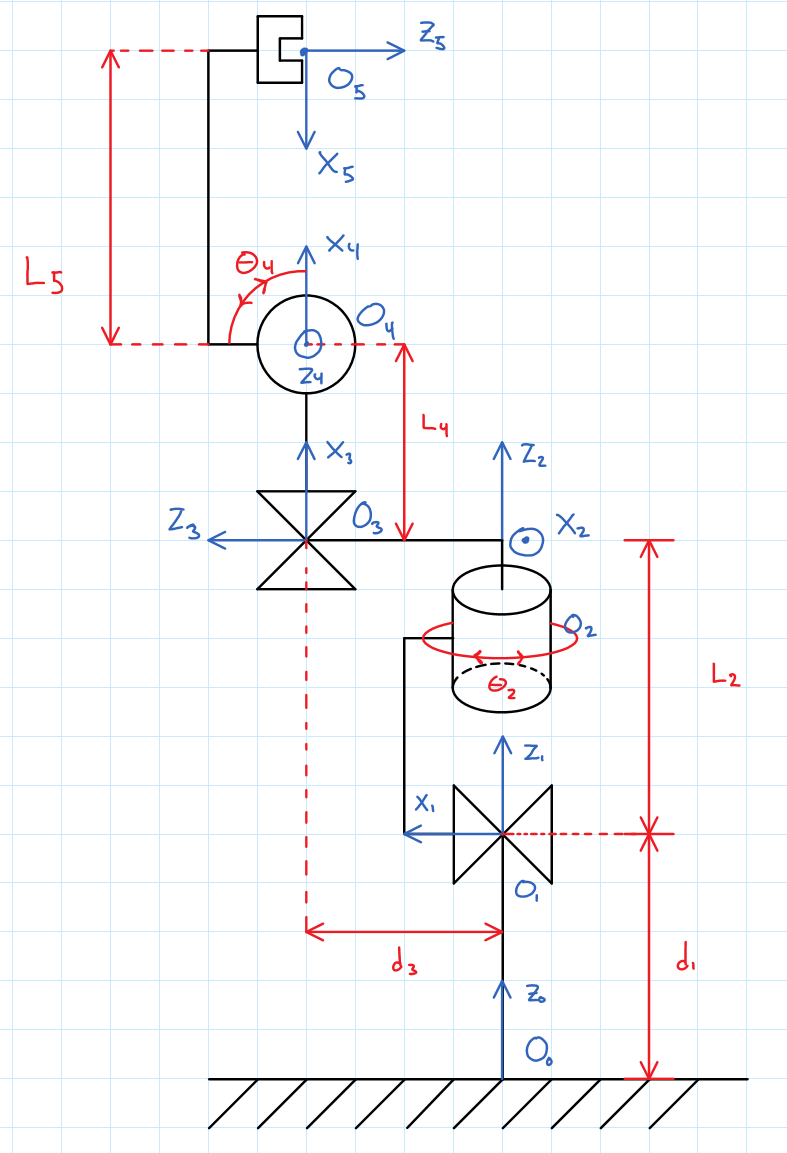
\includegraphics[scale=0.4]{image4}
  \caption{Schematic of the model}
  \label{fig:1}
\end{figure}


According the the schematic, from bottom to top, a prismatic joint is responsible for the height of the seat (along $z_1$). A revolute joint right above it rotate the chair about the $z_2$  so that person sitting on turn their body around their environment. Another prismatic joint moves along $z_3$ axis adjust how far back the backpanel is. Next, a revolute joint rotating about $z_4$ is responsible for adjusting the back angle the person want to sit at. Lastly, we chose the end effector to be the headrest of the chair whose positional state changes if any of the above joint variable changes.
\par
This linkage has 4 degree of freedom, namely translation along z and x, and rotational about z and y in the $O_o$ world reference. The ultimate goal of this linkage is to position the headrest (in turn the back and orientation of the whole chair) in the most comfortable position for the human sitting on it.
\par
A simple case scenario in words is describe below: A human sitting on this chair facing the $-x_0$ direction wants to sit facing forward, while wants to sit higher and lean his back a little bit to the back. Intuitively, if we are to do it, this would translate to the operation on the joint:
\begin{enumerate}
\item joint 2 rotates about $z_2$ by 90 degrees
\item joint 1 moves along $z_1$ by $q_1$ mm
\item joint 4 rotates along $z_4$ by $q_4$ degrees.  
\end{enumerate}

\section{Method}
Based off the schematic in figure 1, we computed the Denavit–Hartenberg parameters, as shown in the following table,
\begin{table}[H]
  \centering
  \begin{tabular}{c|cccc}
i & $\alpha$$_{\text{i-1}}$ & a$_{\text{i-1}}$ & d$_{\text{i}}$ & $\theta$$_{\text{i}}$\\
\hline
1 & 0 & 0 & d$_{\text{1}}$ & 0\\
2 & 0 & 0 & L$_{\text{2}}$ & $\theta_2$+90\\
3 & 90 & 0 & d$_{\text{3}}$ & 90\\
4 & 90 & L$_{\text{4}}$ & 0 & $\theta$$_{\text{4}}$\\
5 & 90 & L$_{\text{5}}$ & 0 & 180\\
\end{tabular}
  \caption{D-H parameters}
\end{table}
where $\vec{q} =
\begin{bmatrix}
  d1 \\ \theta_2 \\ d_3 \\ \theta_4
\end{bmatrix}
$ are joint parameters and $L2 = 450; L4 = 100; L5 = 600$ are the chair constants.
\par
We implement both forward and inverse Kinematics in Matlab, as shown in the following link to GitHub Repository \link{}
\end{document}
%==================================================%
% Bibliography starts here
%==================================================%
% \bibliographystyle{unsrt}
% \bibliography{my_latex_math_template}

%%% Local Variables:
%%% mode: latex
%%% TeX-master: t
%%% End:
